%*----------- SLIDE -------------------------------------------------------------
\begin{frame}[t]{Introdução} 

    No RASC existem diversos projetos de diferentes vertentes da área da robótica, sendo uma delas a dos manipuladores.
    \vspace*{0.3cm}

    Os projetos que compõem essa trilha são:
    %\newline
        \begin{columns}[t]
            \column{.05\linewidth}
            \column{.4\linewidth}
            \begin{itemize}
                \item Walker
                \item Warhog + AUM
                \item Horta-bot
                \item Magician
                \item outros projetos
            \end{itemize}
            \column{.6\linewidth}
            \begin{center}
            %\centerline{
                \begin{figure}
                    % 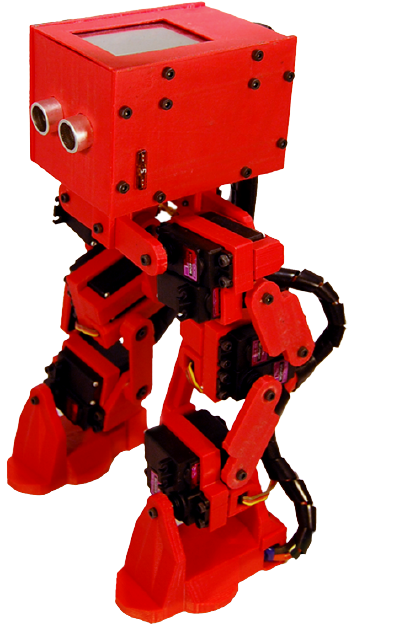
\includegraphics[width=0.3\textwidth]{biped.png}
                \end{figure}
            %}
            \end{center}
        \end{columns}
%*----------- notes
    \note[item]{Notes can help you to remember important information. Turn on the notes option.}
\end{frame}
%-
%*----------- SLIDE -------------------------------------------------------------
\begin{frame}[c]{} 
    % \transdissolve[duration=0.5]
   
    \begin{center}
        \Wider{%
        \begin{shaded}
        \begin{center}
            \vspace*{0.3cm}
            \resizebox{!}{0.6cm}{%
                Walker
            }%
        \end{center}
        \end{shaded}
        }%
    \end{center}
       
%*----------- notes
    \note[item]{Notes can help you to remember important information. Turn on the notes option.}
\end{frame}
%
%*----------- SLIDE -------------------------------------------------------------
\begin{frame}[t]{Objetivo} 
    O projeto consiste em desenvolver um robô de pequeno porte que se desloca sobre dois pés. O robô deve ser capaz de se locomover e desviar de obstáculos em um determinado ambiente.
    \vspace*{0.3cm}

    Materiais do projeto:
   
        \begin{columns}[c]
            \column{.6\textwidth}
                \begin{itemize}
                    \item Board do projeto;
                    \item Simulação do robô
                    \item Estrutura e componentes eletrônicos
                    \item Relatório parcial e apresentações follow-up
                    \item Página no Brazilians in robotics
                \end{itemize}
            \column{.4\textwidth}
                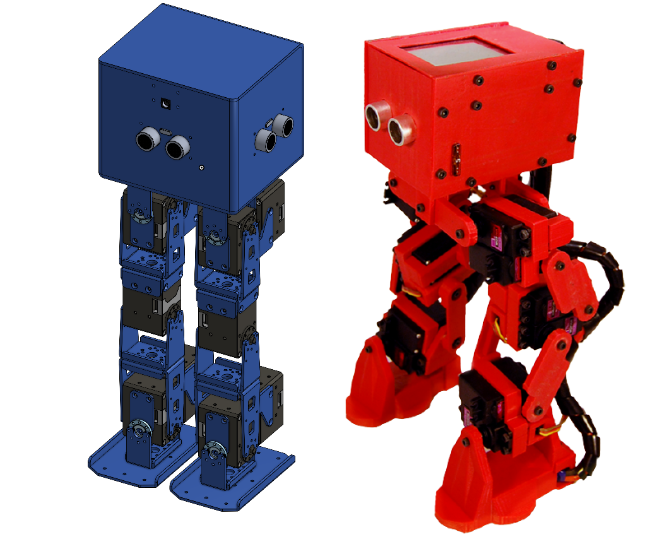
\includegraphics[width=0.8\textwidth]{walker}
        \end{columns}

\end{frame}
%-
%*----------- SLIDE -------------------------------------------------------------
\begin{frame}[c]{} 
    % \transdissolve[duration=0.5]
   
    \begin{center}
        \Wider{%
        \begin{shaded}
        \begin{center}
            \vspace*{0.3cm}
            \resizebox{!}{0.6cm}{%
                Warhog + AUM
            }%
        \end{center}
        \end{shaded}
        }%
    \end{center}
       
%*----------- notes
    \note[item]{Notes can help you to remember important information. Turn on the notes option.}
\end{frame}
%
%*----------- SLIDE -------------------------------------------------------------
\begin{frame}[t]{Objetivo} 
   O objetivo principal deste projeto é desenvolver um modelo para a compensação das perturbações sofridas por manipuladores utilizados em veículos móveis:
   \vspace*{0.3cm}

   Materiais do projeto:
   
        \begin{columns}[c]
            \column{.5\textwidth}
            \begin{itemize}
                \item Board do projeto;
                \item Simulação do robô + manipulador
                \item Estrutura do robô
                \item Página no Brazilians in robotics
            \end{itemize}
            \column{.5\textwidth}
                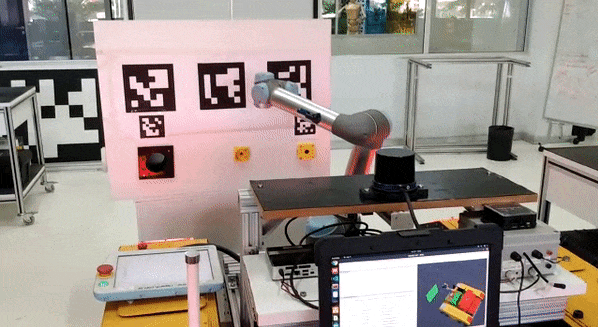
\includegraphics[width=1\textwidth]{warhog+aum.png}
        \end{columns}

\end{frame}
%-
%*----------- SLIDE -------------------------------------------------------------
\begin{frame}[c]{} 
    % \transdissolve[duration=0.5]
   
    \begin{center}
        \Wider{%
        \begin{shaded}
        \begin{center}
            \vspace*{0.3cm}
            \resizebox{!}{0.6cm}{%
                Horta-bot
            }%
        \end{center}
        \end{shaded}
        }%
    \end{center}
       
%*----------- notes
    \note[item]{Notes can help you to remember important information. Turn on the notes option.}
\end{frame}
%
%*----------- SLIDE -------------------------------------------------------------
\begin{frame}[t]{Objetivo} 
    Este projeto consiste em desenvolver um sistema robótico baseado em CNC para deslocamento da unidade de supervisionamento das plantas e do solo.Ele deverá interagir com o ambiente através da dosagem de água, retirada de ervas daninhas, realizar a plantação das hortaliças e atender outras necessidades do sistema.


\end{frame}
%-

%*----------- SLIDE -------------------------------------------------------------
\begin{frame}[c]{} 
    % \transdissolve[duration=0.5]
   
    \begin{center}
        \Wider{%
        \begin{shaded}
        \begin{center}
            \vspace*{0.3cm}
            \resizebox{!}{0.6cm}{%
                Magician
            }%
        \end{center}
        \end{shaded}
        }%
    \end{center}
       
%*----------- notes
    \note[item]{Notes can help you to remember important information. Turn on the notes option.}
\end{frame}
%
%*----------- SLIDE -------------------------------------------------------------
\begin{frame}[t]{Objetivo} 
    Este projeto consiste em implementar as funcionalidades de pick-place e drawing em um robô Dobot Magician.
    \vspace*{0.3cm}

    Materiais do projeto:
        \begin{columns}[c]
            \column{.6\textwidth}
                \begin{itemize}
                    \item Desenvolver algoritmos utilizando ROS;
                    \item Utilizar visão computacional;
                    \item Simular um robô no gazebo;
                    \item Desenvolver habilidades de gestão de projetos.
                \end{itemize}
            \column{.25\textwidth}
                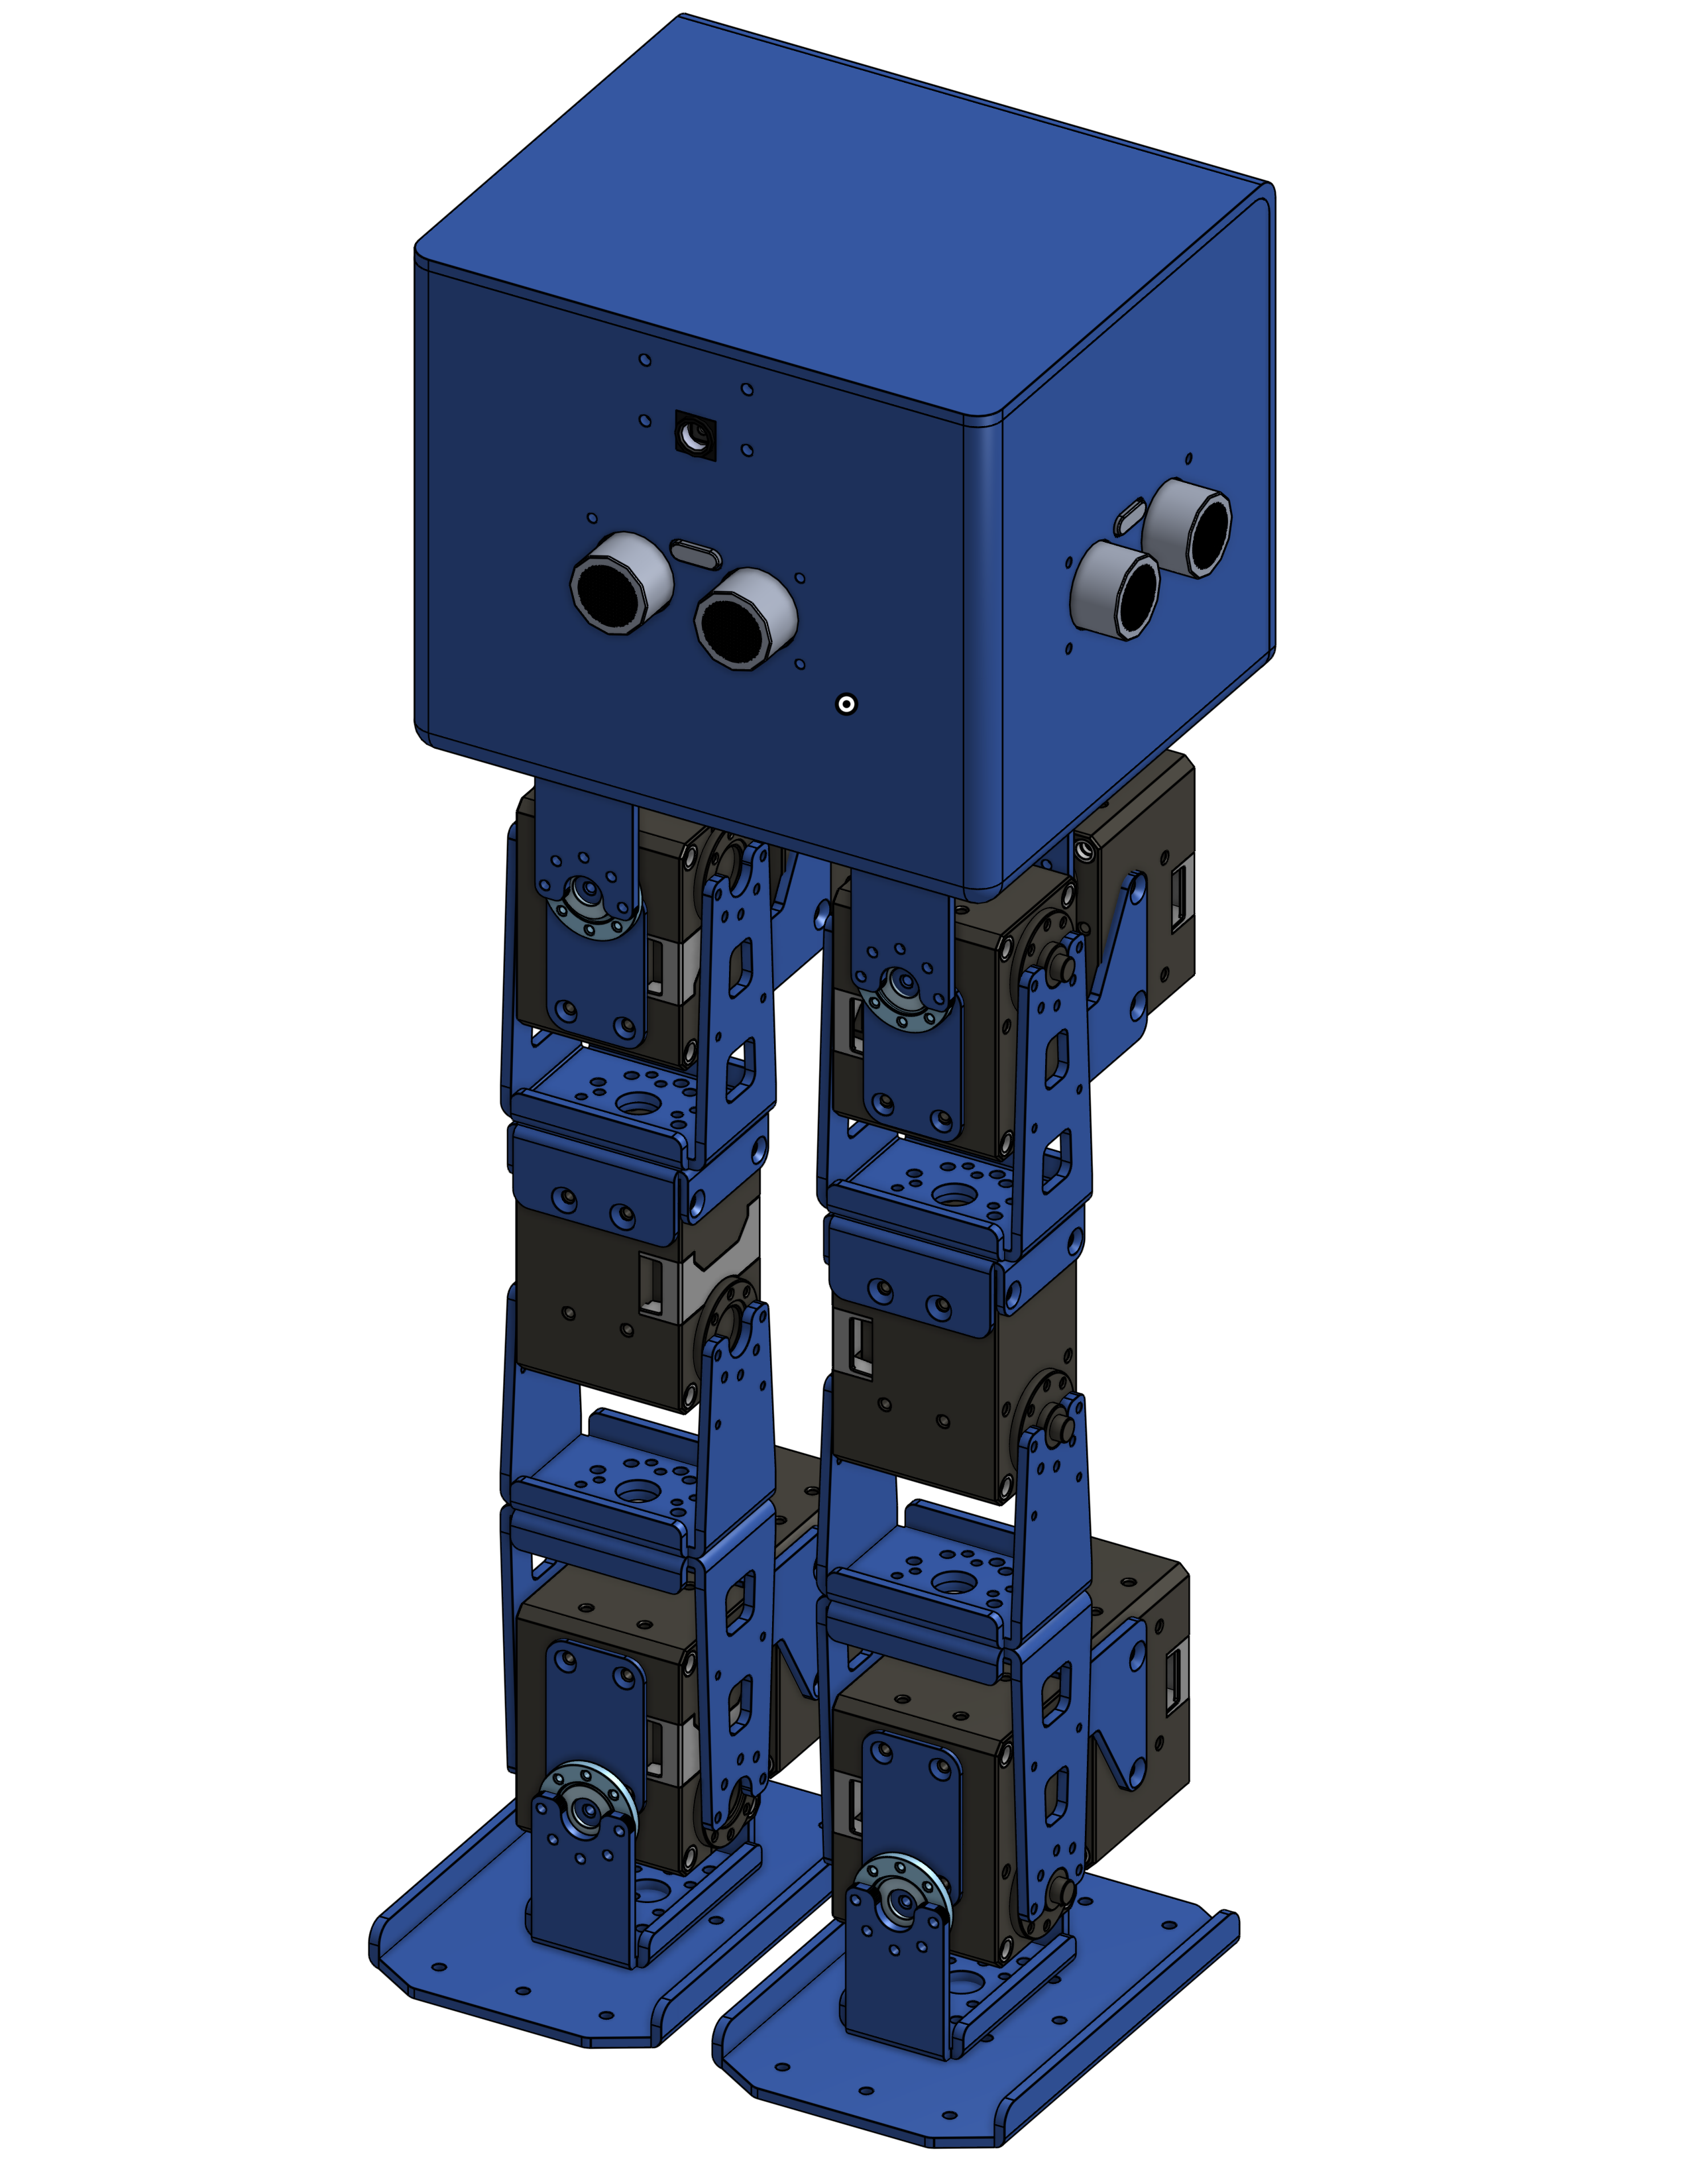
\includegraphics[width=1\textwidth]{walker3D}
        \end{columns}

\end{frame}
%-

%*----------- SLIDE -------------------------------------------------------------
\begin{frame}[c]{} 
    % \transdissolve[duration=0.5]
   
    \begin{center}
        \Wider{%
        \begin{shaded}
        \begin{center}
            \vspace*{0.3cm}
            \resizebox{!}{0.6cm}{%
                outros projetos
            }%
        \end{center}
        \end{shaded}
        }%
    \end{center}
       
%*----------- notes
    \note[item]{Notes can help you to remember important information. Turn on the notes option.}
\end{frame}
%
%*----------- SLIDE -------------------------------------------------------------
\begin{frame}[t]{Objetivos} 
   O objetivo principal destes trabalhos é promover a experiência e o aprendizado dos conhecimentos e ferramentas relacionadas aos robôs manipuladores.
   \vspace*{0.3cm}

    \begin{columns}[c]
         \column{.5\textwidth}
         Projetos:
         \begin{itemize}
          \item Blackthor manipulator
          \item Jax manipulator
         \end{itemize}
         \vspace*{0.3cm}
         Materiais dos projetos:
            \begin{itemize}
                \item Boards dos projetos
                \item Página no Brazilians in robotics
            \end{itemize}
        \column{.5\textwidth}
            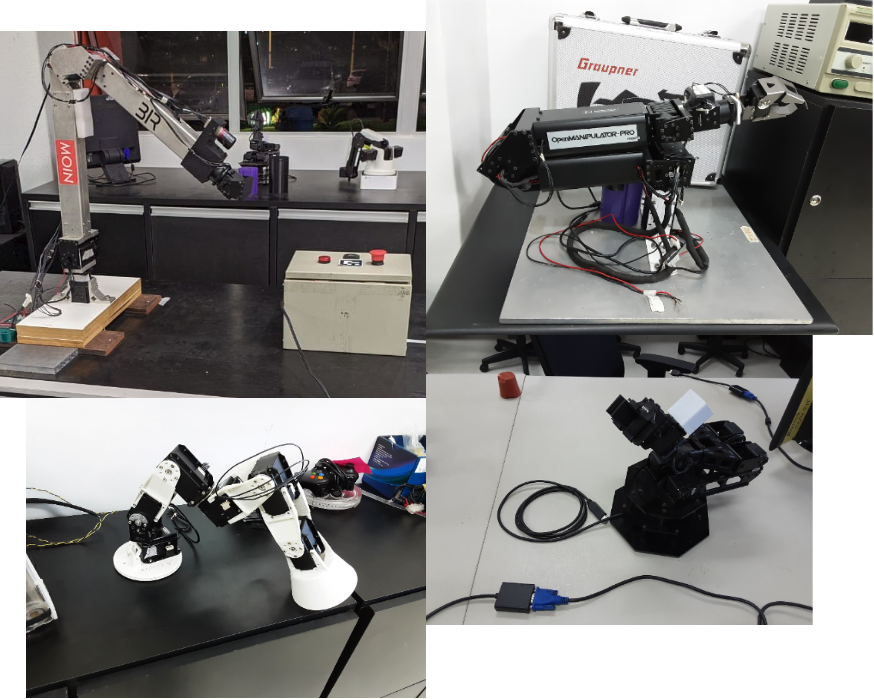
\includegraphics[width=0.85\textwidth]{outros-projetos.png}
    \end{columns}

\end{frame}
%-
%*----------- SLIDE -------------------------------------------------------------
\begin{frame}[c]{} 
    % \transdissolve[duration=0.5]
   
    \begin{center}
        \Wider{%
        \begin{shaded}
        \begin{center}
            \vspace*{0.3cm}
            \resizebox{!}{0.6cm}{%
                Sugestões
            }%
        \end{center}
        \end{shaded}
        }%
    \end{center}
       
%*----------- notes
    \note[item]{Notes can help you to remember important information. Turn on the notes option.}
\end{frame}
%
%*----------- SLIDE -------------------------------------------------------------
\begin{frame}[t]{Sugestões} 

    
    \vspace*{0.3cm}
    \begin{itemize}
        \item Explorar os boards e materiais dos projetos
        \item Ler as páginas e posts dos projetos no brazilians in robotics
        \item Ter contato com os robôs manipuladores do laboratório
    \end{itemize}
    \vspace*{0.8cm}
    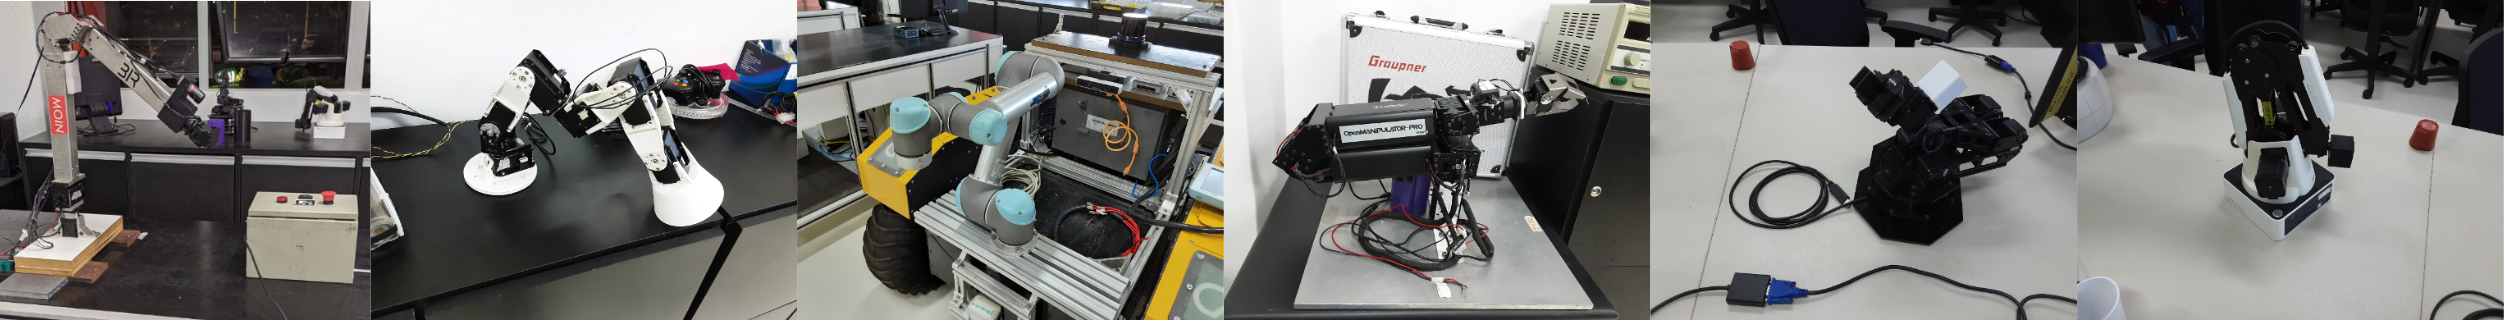
\includegraphics[width=1\textwidth]{projetos-montag.png}
%*----------- notes
    \note[item]{Notes can help you to remember important information. Turn on the notes option.}
\end{frame}
%-